% This is an example of using latex for a paper/report of specified
% size/layout. It's useful if you want to provide a PDF that looks
% like it was made in a normal word processor.

% While writing, don't stop for errors
\nonstopmode

% Use the article doc class, with an 11 pt basic font size
\documentclass[11pt, a4paper]{article}

% Makes the main font Nimbus Roman, a Times New Roman lookalike:
%\usepackage{mathptmx}% http://ctan.org/pkg/mathptmx
% OR use this for proper Times New Roman (from msttcorefonts package
% on Ubuntu). Use xelatex instead of pdflatex to compile:
\usepackage{fontspec}
\usepackage{xltxtra}
\usepackage{xunicode}
\defaultfontfeatures{Scale=MatchLowercase,Mapping=tex-text}
\setmainfont{Times New Roman}

% Nice citations
\usepackage{natbib}

% Set margins
\usepackage[margin=2.5cm]{geometry}

% Multilingual support
\usepackage[english]{babel}

% Nice mathematics
\usepackage{amsmath}

% Left right harpoons for kinetic equations
\usepackage{mathtools}

% Control over maketitle
\usepackage{titling}

% Section styling
\usepackage{titlesec}

% Ability to use colour in text
\usepackage[usenames]{color}
\definecolor{grey}{rgb}{0.6, 0.6, 0.63}
\definecolor{black}{rgb}{0, 0, 0}

% For the \degree symbol
\usepackage{gensymb}

% Allow includegraphics and nice wrapped figures
\usepackage{graphicx}
\usepackage{wrapfig}
\usepackage[outercaption]{sidecap}
\usepackage{subfigure}

% Nice quotes
\usepackage{csquotes}

% Set formats using titlesec
\titleformat*{\section}{\bfseries\rmfamily}
\titleformat*{\subsection}{\bfseries\itshape\rmfamily}

% thetitle is the number of the section. This sets the distance from
% the number to the section text.
\titlelabel{\thetitle.\hskip0.3em\relax}

% Set title spacing with titlesec, too.  The first {1.0ex plus .2ex
% minus .7ex} sets the spacing above the section title. The second
% {-1.0ex plus 0.2ex} sets the spacing the section title to the
% paragraph.
\titlespacing{\section}{0pc}{1.0ex plus .2ex minus .7ex}{-1.1ex plus 0.2ex}

%% Trick to define a language alias and permit language = {en} in the .bib file.
% From: http://tex.stackexchange.com/questions/199254/babel-define-language-synonym
\usepackage{letltxmacro}
\LetLtxMacro{\ORIGselectlanguage}{\selectlanguage}
\makeatletter
\DeclareRobustCommand{\selectlanguage}[1]{%
  \@ifundefined{alias@\string#1}
    {\ORIGselectlanguage{#1}}
    {\begingroup\edef\x{\endgroup
       \noexpand\ORIGselectlanguage{\@nameuse{alias@#1}}}\x}%
}
\newcommand{\definelanguagealias}[2]{%
  \@namedef{alias@#1}{#2}%
}
\makeatother
\definelanguagealias{en}{english}
\definelanguagealias{eng}{english}
%% End language alias trick

%% Any aliases here
\newcommand{\mb}[1]{\mathbf{#1}} % this won't work?
% Emphasis and bold.
\newcommand{\e}{\emph}
\newcommand{\code}[1]{\textsf{#1}}
\newcommand{\dvrg}{\nabla\vcdot\nabla}
%% END aliases

% Custom font defs
% fontsize is \fontsize{fontsize}{linespacesize}
\def\authorListFont{\fontsize{11}{11} }
\def\corrAuthorFont{\fontsize{10}{10} }
\def\affiliationListFont{\fontsize{11}{11}\itshape }
\def\titleFont{\fontsize{14}{11} \bfseries }
\def\textFont{\fontsize{11}{11} }
\def\sectionHdrFont{\fontsize{11}{11}\bfseries}
\def\bibFont{\fontsize{10}{10} }
\def\captionFont{\fontsize{10}{10} }

% Caption font size to be small.
\usepackage[font=small,labelfont=bf]{caption}

% Make a dot for the dot product, call it vcdot for 'vector calculus
% dot'. Bigger than \cdot, smaller than \bullet.
\makeatletter
\newcommand*\vcdot{\mathpalette\vcdot@{.35}}
\newcommand*\vcdot@[2]{\mathbin{\vcenter{\hbox{\scalebox{#2}{$\m@th#1\bullet$}}}}}
\makeatother

\def\firstAuthorLast{James}

% Affiliations
\def\Address{\\
\affiliationListFont Adaptive Behaviour Research Group, Department of Psychology,
  The University of Sheffield, Sheffield, UK \\
}

% The Corresponding Author should be marked with an asterisk. Provide
% the exact contact address (this time including street name and city
% zip code) and email of the corresponding author
\def\corrAuthor{Seb James}
\def\corrAddress{Department of Psychology, The University of Sheffield,
  Western Bank, Sheffield, S10 2TP, UK}
\def\corrEmail{seb.james@sheffield.ac.uk}

% Figure out the font for the author list..
\def\Authors{\authorListFont Sebastian~S.~James, Stuart~P.~Wilson  \Address \\
  \corrAuthorFont $^{*}$ Correspondence: \corrEmail}

% No page numbering please
\pagenumbering{gobble}

% A trick to get the bibliography to show up with 1. 2. etc in place
% of [1], [2] etc.:
\makeatletter
\renewcommand\@biblabel[1]{#1.}
\makeatother

% reduce separation between bibliography items if not using natbib:
\let\OLDthebibliography\thebibliography
\renewcommand\thebibliography[1]{
  \OLDthebibliography{#1}
  \setlength{\parskip}{0pt}
  \setlength{\itemsep}{0pt plus 0.3ex}
}

% Set correct font for bibliography (doesn't work yet)
%\renewcommand*{\bibfont}{\bibFont}

% No paragraph indenting to match the VPH format
\setlength{\parindent}{0pt}

% Skip a line after paragraphs
\setlength{\parskip}{0.5\baselineskip}
\onecolumn

% titling definitions
\pretitle{\begin{center}\titleFont}
\posttitle{\par\end{center}\vskip 0em}
\preauthor{ % Fonts are set within \Authors
        \vspace{-1.1cm} % Bring authors up towards title
        \begin{center}
        \begin{tabular}[t]{c}
}
\postauthor{\end{tabular}\par\end{center}}

% Define title, empty date and authors
\title {
%  Competition can account for stopping in a gradient-following model
%  of the retinotectal projection \\
%  \emph{or} \\
%  Competition provides stopping for the chemoaffinity
%  theory which is robust to noise \\
%  \emph{or} \\
%  Self-organisation of topographically ordered axon connections can take place
%  in a noisy environment if axons compete \\
%  \emph{or} \\
Time to stop; agent-based modelling of chemoaffinity with competition
}
\date{} % No date please
\author{\Authors}

% Simplified chemoaffinity explains retinotectal mapping via local axon-axon
% interactions
%
% Focus on the chemoaffinity idea for this model. Show that local interactions
% can provide an account for growth cones finding their targets.

%% END OF PREAMBLE

\begin{document}

\setlength{\droptitle}{-1.8cm} % move the title up a suitable amount
\maketitle

\vspace{-1.8cm} % HACK bring the introduction up towards the title. It
                % would be better to do this with titling in \maketitle

% Note this is the SfN draft abstract, and will need rewriting.
\emph{In the classic Chemoaffinity theory, the retinotectal axon projection is
thought to use pairs of orthogonal signalling gradients in the retina to
specify the eventual location of synapses made on the surface of the
tectum/superior colliculus. Similar orthogonal gradients in the tectum provide
a coordinate system which allows the axons to match their prespecified
destination with the correct location. Although the Ephrins have been shown to
guide axons toward their destination, there has yet to emerge a complete
account of the local interactions which halt the axonal growth cones in the
correct locations to recreate the topography of the retinal cells. The model
of \citet{simpson_simple_2011} provides an account of the basic topographic
arrangement of cells on the tectum, as well as reproducing well known surgical
and genetic manipulation experiments. However, it suffers from the absence of
a local chemotactic guidance mechanism. Instead, each agent in that model is
given instantaneous knowledge of the vector that would move it toward its
pre-specified destination. In addition to the globally supervised
chemoaffinity term, \citet{simpson_simple_2011} introduced a competitive
interaction for space between growth cone agents and a receptor-receptor
axon-axon interaction in order to account for the full set of experimental
manipulations. Here, we propose the replacement of the chemoaffinity term with
a gradient following model consisting of axonal growth cone agents which carry
receptor molecule expression determined by their soma's location of origin on
the retina. Growth cones move on the simulated tectum guided by two pairs of
opposing, orthogonal signalling molecules representing the Ephrin ligands. We
show that with only the receptor-ligand mediated chemoaffinity term and a
receptor-receptor based axon-axon interaction term (meaning that all growth
cone interactions are communicated by receptor signalling), a full range of
experimental manipulations to the retinotectal system can be
reproduced. Furthermore, we show that the observation that competition is not
an essential requirement for axons to find their
way \citep{gosse_retinotopic_2008} is also accounted for by the model, due to
the opposing influences of signalling gradient pairs. Finally, we demonstrate
that, assuming exponentially varying receptor expression in the retina, tectal
ligand expression should either be exponential if the receptor-ligand signal
induces repulsion (i.e. gradient descent) or logarithmic if the signal induces
attraction (gradient ascent). Thus, we find that a model analogous to the one
we presented in \citet{james_modelling_2020} that accounts for murine barrel
patterning is also a candidate mechanism for the arrangement of the more
continuous retinotectal system.}

%%%%%%%%%%%%%%%%%%%%%%%%%%%%%%%%%%%%%%%%%%%%%%%%%%%%%%%%%%%%%%%%%%%%%%%%%%%%%%%
\section{Introduction}

The retinotectal projection has been an important model system in the study of
how the cells of the central nervous system are accurately connected together
into functional networks. This projection connects the light-gathering cells
in the retina to movement-related cells in the optic tectum (known as the
superior colliculus in mammals). Light sources originating close to each other
in the environment tend to activate retinal ganglion cells (either
directly \cite{iRGC_citation} or indirectly via rods and cones) situated close
together in the eye so that an image of the environment is formed on the
retinal surface. It has been discovered that the topography of the retina is
preserved within brain regions that process this information such that cells
which are adjacent within the retina primarily excite cells adjacent in the
tectum. This indicates that during development there must exist a mechanism
which ensures the correct arrangement of the axons which leave the retina and
connect to cells in the tectum.

One reason for the success of the study of the retinotectal projection is its
capacity to be experimentally manipulated. In some non-mammalian species, both
the retina and the tectum can be partially ablated, or even physically
reorganised in-vivo, after which axons regrow to restore the order and
function of the system for the individual animal. This manipulability was
exploited in influential work by R. W. Sperry and co-workers during the
mid-twentieth century, leading to Sperry's 1963 summary of
the \emph{chemoaffinity theory} \citep{sperry_chemoaffinity_1963} which
proposes the existence of morphogenetic gradients that guide axons to their
destination. The chemoaffinity theory was given robust support by the
discovery of the ephrin ligands and their receptors \citep{cheng_complementary_1995,drescher_vitro_1995}
which have been shown to form into graded expression fields in the
retina \citep{braisted_graded_1997}, tectum \citep{braisted_graded_1997,feldheim_genetic_2000} as well as in other
sensory systems, such as the somatosensory
system \citep{vanderhaeghen_mapping_2000}. The Ephrin ligands have a clear
effect on axonal outgrowth, as shown in in-vitro \citep{cheng_complementary_1995,drescher_vitro_1995,hansen_retinal_2004} and
in-vivo \citep{frisen_ephrin-a5_1998,rodger_transient_2000,mann_topographic_2002,hindges_ephb_2002} studies.
%
% A-P:
%
% EphA and ephrinAs: Anteroposterior axis of retiontectal projection
% (Nasal-Temporal on retina; Anteroposterior on tectum).
%
% RGM (tectum) Neogenin (retina)
%
% D-V:
%
% EphB and ephrin B: Dorsoventral on retina; dorsoventral on tectum.
%
% En-2: Repels temporal growth cones of xenopus ret-tec axons and attracts
% nasal ones. Brunet et all, Nature, 2005
%
% Ryk/Fz (retina) and Wnt3 (tectum) (Flanahan, 2006)
%

It is tempting to consider the retinotectal projection well understood. With a
comprehensive theory supported by a biochemical mechanism, is there anything
left to understand? That question can be answered by reviewing retinotectal
modelling papers.

Mini-review here, which contrasts some of the modelling papers. The upshot is
that a central problem with models is not how the axons know how to get closer
to their destination, but how they know they have \emph{arrived} at their true
destination. Also make the point that many of the models are phenomenological
in nature and do not elucidate the mechanisms behind the arrangement.

In a recent paper, we proposed a self-organising mechanism, based on
morphogenetic signalling gradients, which can arrange
axons growing from the thalamus to the somatosensory cortex into the well
known murine barrel cortex pattern~\citep{james_modelling_2020}. In
characterising that system, we explored the effect of various types of
noise. We found that the mechanism was robust to noise in the expression of
the signalling molecules over a wide range of amplitudes and length-scales,
and that noise in the interaction parameters, which are obtained by sampling
the signalling molecules in the source tissue (the thalamic barreloid field)
could cause topological defects. The question of noise in axon guidance has
been explored by \citet{goodhill_can_2016}.

\color{grey}
\textbf{New introduction:} Simpson and Goodhill presented a model in which the
chemoaffinity mechanism is non-biological. We offer a model in which a
competition mechanism counteracts the drive of axons along the ephrin
gradient. Will we need the axon-axon interaction mechanism based on
non-same-Eph repulsion?

\textbf{Another approach:} We present a model of gradient-following based on graded
interactions between the growth cones of retinal ganglion cell axons and the
tectal surface. We show that a combination of exponentially graded expression
in the retina \citep{reber_relative_2004} and exponentially (for repulsively
interacting receptor ligand pairs) \emph{or} logarithmically (for attractively
interacting receptor/ligands) graded expression on the tectum permits a purely
local model to reproduce the majority of reported phenomena associated with
retinotectal organisation.

There have been many approaches to modelling the organisation of the
retinotectal projection. Many of these models are wholly or partially
phenomenological.

A model which carefully deals with receptor
binding is given by \citet{naoki_revisiting_2017} \citep[see also][]{mortimer_bayesian_2009}.

Gradient based models: \citet{nakamoto_topographically_1996}

\color{black}
\section{Results}

\subsection*{Chemoaffinity as the sole patterning mechanism}

The first question we tried to answer was whether a gradient following
mechanism, acting alone, is sufficient to pattern the tectum. To do so, we
simulated the retina and tectum as unit square regions and defined retinal
receptor expression and tectal ligand expression across these squares
(Fig.\,\ref{f:ex}).

\begin{figure}
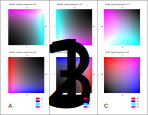
\includegraphics[width=\linewidth]{./images/expressions_fig.png}
\caption{Simulated retinal and tectal signalling molecule expression. Four
receptor types are expressed, and four corresponding ligand types. Receptors
of type $i$ are activated by ligands of type $i$.
%
\textbf{A} Retinal receptor expression, $r_i$. Four receptors are expressed and
displayed here in two dual-colour maps. $r_0$ and $r_1$ are red and blue;
$r_2$ and $r_3$ are cyan and magenta. $r_0$ increases as an exponential
function of $-x$; $r_1$ increases with an exponential function of $-y$. $r_2$
and $r_3$ have the opposite sense. Retinal receptor expression is modelled
with exponential functions because there is ample evidence to support this
form. $N$: nasal, $T$: temporal, $D$: dorsal, $V$: ventral.
%
\textbf{B} Retinal ligand expression, $l_i$, is expressed in complimentary
gradients \citep{hornberger_modulation_1999}.
%
\textbf{C} Tectal ligand expression $L_i$. Tectal ligand expression is shown in a linear form,
as there is less evidence to determine whether ligand expression is
exponential, linear or logarithmic on the tectum.
$L$: lateral, $M$: medial, $C$: caudal, $R$: rostral.
}
\label{f:ex}
\end{figure}

Each retinal ganglion cell projects growth cones (referred to
as \emph{branches}) which carry a set of 4 receptors, $r_i$ indexed by $i$ and
expressed at levels determined by the cell soma's location on the
retina. (Four ligands, $l_i$, are also expressed by RGCs, but these are not
used by the chemoaffinity simulation.) The expression levels of the receptors
vary with respect to the soma's position on the retinal surface. Each receptor
varies only with respect to one dimension.  Receptor expression gradients are
arranged in orthogonal pairs with the gradient of $r_0$ being orthogonal to
that of $r_1$. $r_2$, whose gradient is opposite to $r_0$, is orthogonal to
$r_3$.

Because there is convincing evidence that EphA and EphB receptors are
expressed in exponentially increasing
patterns \citep{reber_relative_2004,feldheim_genetic_2000,brown_topographic_2000,koulakov_stochastic_2004},
we use an exponential form for retinal receptor expressions, in common with
other modelling
studies~\citep{reber_relative_2004,koulakov_stochastic_2004,simpson_simple_2011}.
We adopt the same precise form for the retinal receptor expression
as \citet{simpson_simple_2011} which is
\begin{equation} \label{e:retrcpt}
r_i(x,y) = 1.05 + 0.26 \exp(2.3 x)
\end{equation}
for even values of $i$. The opposing expressions (for even values of $i$)
are given by substituting $(1-x)$ for $x$.

The tectum expresses ligands, $L_i$, for the retinal receptors, also
in orthogonal pairs of gradients. Although several studies model tectal ligand
expression with exponential functions \citep{koulakov_stochastic_2004}, the
experimental evidence for ligand expression is more ambiguous than that for
retinal receptor expression (Supp.~Fig
\textbf{XXXXX}). We kept in mind the possibility that tectal ligand
expression may be modelled by exponential, linear or logarithmic functions,
but initially, we set it to the function
\begin{equation} \label{e:tecligexp}
L_i^{\text{exp}}(x,y) = 1.05 + 0.26 \exp(2.3 x)
\end{equation}
for odd values of $i$ and using the same substitution of $(1-x)$ for $x$ to
obtain the opposing ligand expressions for $i$ even.

While we do not explicitly name $r_0$, $r_1$,
etc.~as \emph{EphA}, \emph{EphB}, the suggestion is that $r$ includes EphA,
EphB, Ryk \citep{schmitt_wntryk_2006} and
Neogenin \citep{rajagopalan_neogenin_2004} receptors and that $L$ includes the
ephrin-A, ephrin-B, Wnt3 \citep{schmitt_wntryk_2006} and
RGM \citep{monnier_rgm_2002} ligands, each of which has been shown to play a
r\^ole in retinotectal map formation.

Figure~\ref{f:ex} shows colour maps of receptor and ligand
expression. Coordinates within the simulated retina and tectum are normalised,
with 1 corresponding to 2 mm on the tectum and on the retina for
mouse \citep{reber_relative_2004}.

\color{grey}
This means that growth cones of approximate
radius 5 $\mu$m = 0.005 mm \citep{goodhill_can_2016} have a radius $r$ =
0.0025 in the arbitrary units of the simulation. For a realistic simulation
based on mouse, the approximate RGC density in the retina is around 44000
cells per retina \citep{jeon_major_1998}. This sets the side length of the
retina to $\sqrt{44000} \approx 200$. This results in a simulation of
prodigious computational size, which although tractable (10 s per step,
requiring several hours, rather than days to run) is not convenient. To
maintain the relationship between growth cone size and cell density, we permit
a smaller number of growth cones ($400\times8=3200$) but keep the fractional
area of the branches at 0.86 ($44000 \times \pi r^2$) (if there is one cone
per axon) or 6.9 (if there are 8 cones per axon).

\color{black}
Each discrete element in Fig.\,\ref{f:ex}B projects one RGC axon with 4
branches to the tectum, carrying the receptor expression at the retinal
element's location.
At each timestep in a simulation, the position, $\mathbf{x}_{b,t}$, at time
$t$ of each branch $b$ is updated according to
%
\begin{equation}
\mathbf{x}_{b,t+1} = \mathbf{x}_{b,t} + \mathbf{M}_{b}
\end{equation}
%
where $\mathbf{M}_{b}$, the movement vector, is the sum of a chemoaffinity
effect and a `border effect', $\mathbf{B}_b$, which acts to retain branches
within the tectal region:
%
\begin{equation} \label{e:mv}
\mathbf{M}_{b} = m_{\!_G} \mathbf{G}_b + 0.5 \mathbf{B}_b
\end{equation}
%
evaluated at time $t$.

% G - chemoaffinity description
%\subsection{Chemoaffinity}
The chemoaffinity component, $\mathbf{G}_b$, is governed by receptor-ligand
signalling. The signal transmitted when a tectal ligand binds to a RGC
receptor on a branch (forward signalling) can lead to one of two effects; the
signal may induce an attraction towards the ligand-expressing region or a
repulsion away from it.
%
For axon-tectum interactions, we implemented attraction as a climbing of the
tectal ligand expression gradient and repulsion as gradient descent.
%
To determine the strength of the effect we assumed a purely linear receptor
binding model, and set the chemotactic movement vector of the branch $b$ at
location $\mathbf{x}_b$ on the tectum to be
%
\begin{equation}
\mathbf{G}_b = \sum_i^N F_i\,r_{i,b} \nabla L_i(\mathbf{x}_b)
\end{equation}
%
where $r_{i,b}$ is the receptor expression on branch $b$ for ligand-receptor
pair $i$, $\nabla L_i$ is the gradient of expression of ligand $i$ on the
tectum and $F_i$ denotes the direction of the interaction induced when a
molecule of ligand $i$ binds to a receptor $i$ molecule. $F_i$ takes the value
-1 for a repulsive interaction or 1 for an attractive interaction.
%
We assumed that all
receptor-ligand signalled interactions are repulsive ($F_i=-1, \forall i$), as
for EphA-ephrinA
coupling \citep{drescher_vitro_1995,nakamoto_topographically_1996}.
%
$m_{\!_G}$ is a
scalar parameter which controls how much movement is generated for a given
receptor-ligand signal size.
% end chemoaffinity description

% \subsection{Border effect} % border effect description
The border effect is also based on gradient following by assuming that
there is some other molecular signal which acts on all branches near the
boundary of the tectal tissue. For a branch with position $(x,y)$, $\mathbf{B}_b$ is
given by:
%
\begin{equation}
B_{b,x} = \begin{cases}
        r-x      & x<r \\
        1-r-x    & x>1-r
\end{cases}
B_{b,y} = \begin{cases}
        r-y      & y<r \\
        1-r-y    & y>1-r
\end{cases}
\end{equation}
%
Thus $\mathbf{B}_b$ is equivalent to the action of a repulsive signalling
molecule expressed around the border of the tectum, whose expression increases
quadratically outside the tectum and affects any branch touching (or outside)
the boundary.
% end border effect description

% \subsection*{Initial conditions}
Branches were initially randomly distributed in a stripe at the rostral side
of the tectum at the start of each simulation. Each RGC axon was assigned a
random initial position coordinate:
\begin{equation}
\mathbf{x}_{\text{axon},t=0} = (U(0,1), U(-0.2,0))
\end{equation}
where U(p,q) is a number selected from a random uniform distribution in the
range $[p,q)$. Each of the 4 branches per RGC axon was given its parent
axon's initial position, plus a randomly generated offset with coordinates
derived from a normal distribution of mean 0 and standard deviation 0.1.
% end initial conditions

The results of running this simulation for 300 time steps are shown in
Fig.\,\ref{f:ch}. Fig.\,\ref{f:ch}A indicates the colour code used for retinal
cell position; dorsal retinal cells are indicated by green, nasal cells by
red. Lightness gives position along the relevant axis so that cells at the
dorsal-nasal corner are yellow and those at the ventral-transverse corner are
black. Fig.\,\ref{f:ch}E shows the expected layout of retinal ganglion cell
axons on the tectum. The axons retain the colour of their originating cell on
the retina, as shown in Fig.\,\ref{f:ch}A. Nasal cell axons should be arranged
caudally; dorsal axons laterally; axons should be evenly spaced and the
pattern should span the entire tectum.  Fig.\,\ref{f:ch}B--D show `fish net'
plots of the axon centroids at three timepoints. An axon's centroid is the
average location of its 4 branches. In these plots, lines are drawn between
axons that are expected to arrange themselves adjacently to one another by the
end of the simulation. The number of line crossings in this plot gives an
indication of the disorder in the arrangement. Fig.\,\ref{f:ch}G shows the
positions of the individual branches (i.e.~growth cones) at $t=300$ that
contribute to the the plot in Fig.\,\ref{f:ch}D. By this time, the topological
order matches that shown in Fig.\,\ref{f:ch}E. Opposing gradients have sorted
the axons along the two axes to form a grid of cells. However, the arrangement
does not span the full tectum. Fig.\,\ref{f:ch}F shows two pattern
metrics. The first metric, $\epsilon$, is the sum of squared distance errors
of the axon centroids, with $\mathbf{x}_{k}$, the location of the centroid of
the branches of axon $k$ and $\mathbf{x}'_{k}$ the target tectal location for
axon $k$:
%
\begin{equation}\label{e:eps}
\epsilon = \sum_k |\mathbf{x}_{k} - \mathbf{x}'_{k}|^2.
\end{equation}
%
$\epsilon$ tends to 0 as the pattern approaches the target layout. However,
two patterns may have the same non-zero value for $\epsilon$, despite one
being qualitatively more disordered than the other. For this reason, we also
use the number of crossings in the fish net plot of Fig.\,\ref{f:ch}D as a
second metric, called $\eta$. The expected number of crossings in the wildtype
pattern is 0, as in Fig.\,\ref{f:ch}E, although note that in some patterns,
the expected number of crossings is non-zero. Fig.\,\ref{f:ch}H shows selected
axons (one from the centre and one from each corner of the retina) and their
position history.

% ./build/sim/agent/agent1 configs/simpler/m_ee_G.json configs/simpler/e_wt_fig2.json
\begin{figure}
\includegraphics[width=\linewidth]{./images/j4_ee_G_wt_fig2.png}
\caption{The pure gradient-following model.}
\label{f:ch}
\end{figure}

The form of the retinal receptor expression (Eq.\,\ref{e:retrcpt}) is based on
empirical measurement, but the tectal ligand expression
(Eq.\,\ref{e:tecligexp}) was chosen arbitrarily. To expand the pattern in
Fig.\,\ref{f:ch}D so that it covers the entire tectum, we needed only to
adjust the tectal ligand expression, substituting the alternative exponential
expression:
%
\begin{equation} \label{e:tecligexp2}
L_i^{\text{exp}}(x,y) = 1.05 + 0.26 \exp(1.1 x)
\end{equation}
%
for the tectal ligand expression.

The result at $t=300$ is shown in Figs.\,\ref{f:chalt}A and \ref{f:chalt}B. The
axon centroids are arranged across the full tectal surface.  The arrangement
is slightly disordered around the middle of the tectum. This is caused by
numerical artefacts from the discretization of the ligand expression and the
fact that in the centre, the difference between the opposing receptor-ligand
signals is very small. Nevertheless, the result demonstrates that a modified
form for the tectal ligand expression (which was found easily by hand tuning)
allows a well ordered map to form for the wildtype system. Fig
.\,\ref{f:chalt}C shows the error metric (\textbf{FIXIMAGE}), $\epsilon$,
which is much closer to 0 with the new ligand expression.

% ./build/sim/agent/agent1 configs/simpler/m_eE_G.json  configs/simpler/e_wt_fig2.json
\begin{figure}
\includegraphics[width=\linewidth]{./images/j4_eE_G_wt_fig3.png}
\caption{The pure gradient-following model (alt exponential).}
\label{f:chalt}
\end{figure}

This `chemoaffinity only' model begins to encounter problems when we introduce
simulations of experimental surgical manipulations. Simulated surgery is
performed by manipulating the maps shown in
Fig.\,\ref{f:ex}. Fig.\,\ref{f:trot90} shows the expression maps and the
resulting gradients that result from the surgical manipulation in which a
graft of the tectum is rotated by a quarter turn and replaced. We rotate an
8x8 square of the tectum and then recompute the gradients. As the ligand
expression is discretize rather than continuous, we compute the gradient
numerically, with the gradient in direction $x$ computed as the difference
between the expression of the two neighbouring elements divided by twice the
element distance. As there are four ligands expressed on the tectum, there are
four pairs of gradient maps, each of which is shown in Fig.\,\ref{f:trot90}.

% Visualisation of ligand expression and gradients on the tectum for the
% graft-rotate 90 degrees simulated surgical manipulation
% ./build/sim/agent/tissuevis configs/simpler/m_eE_G.json configs/simpler/e_tecrot90_fig4row1.json
%
\begin{figure}
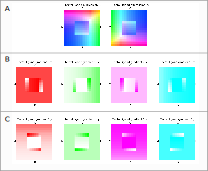
\includegraphics[width=\linewidth]{./images/Tissuevisb.png}
\caption{Ligand expression and gradients on the tectum for the
graft-rotate 90 degrees simulated surgical manipulation}
\label{f:trot90}
\end{figure}

Fig.\,\ref{f:tmanip} shows the tectal ligand expression for ligands $L_1$ and
$L_2$ for the five other surgical manipulations applied in this work. These
are a 180\degree~rotation (Fig\,\ref{f:tmanip}A), a graft-swap manipulation
(Fig\,\ref{f:tmanip}B), ablation of half the retina (Fig\,\ref{f:tmanip}C),
and ablation of half the tectum (Fig\,\ref{f:tmanip}D). A mismatch
manipulation was also performed in which which half of the retina is removed
along with the half of the tectum to which the remaining retina would project.

\begin{figure}

\includegraphics[width=\linewidth]{./images/expressions_manipulations.png}
\caption{Ligand expression and gradients on the tectum for the
other simulated surgical manipulations}
\label{f:tmanip}
\end{figure}

Fig\,\ref{f:chsurg} shows the results of 6 simulated surgical
manipulations. In row A, a patch of tectal tissue has been cut out and rotated
by a quarter turn, as in Fig.\,\ref{f:trot90}. From left to right, graphs show
i) the expected final layout of the tectum, according to the results of
experimental work, with the colour code giving the origin location of the
axon's soma on the retina, ii) The locations of individual axon branches at
simulation end, iii) the centroids of each axons' branches and iv) a rather
useless selected axons box \textbf{FIXME}. Simulation time was 1000 time steps. The final
locations of branches and axon centroids indicates that a qualitative rotation
of the graft patch has occurred, with red branches inside the patch being
located at the lateral-caudal corner rather than the medial-caudal corner. A
portion of the graft region (the medial side, after rotation) is free of
branches, indicating that the pattern is partial. A similar result is seen for
the 180\degree~example in row B, in which the caudal half of the rotated patch
is free of branches, but the rostral half contains branches with the correctly
rotated orientations.

Fig.\,\ref{f:chsurg}C shows the result of the patch swap manipulation, in
which 12x4 element grafts, one from the caudal side of the tectum and one from
the rostral side are swapped. This simulation is unsuccessful in patterning
the caudal half of the tectum. The large gradients, both positive and
negative, caused by the discontinuities along the long edges of the grafts
attracts almost all the branches (whose initial position is the rostral edge)
and very few pass through to the caudal side.

The retinal ablation shown in Fig.\,\ref{f:chsurg}D is also unsuccessful, with
the axons from the surviving nasal retina (the transverse half was removed)
failing to arrange themselves across the entire tectum, due to the pure
`position specification' which the dual gradient model achieves. Similarly,
the tectal ablation simulation fails to reproduce experimentally observed
results in which the retinal map `squashes up' within the remaining tectal
region. Instead, axons from the transverse retina arrange with normal spacing
and axons from the nasal retina are pushd to the caudal-most side of the
remaining tectum (Fig.\,\ref{f:chsurg}E). A similar result occurs in the
mismatch experiment (Fig.\,\ref{f:chsurg}F), but in this case there are no
axons from teh transverse retina, which was been ablated and only the axons
from the nasal retina are present, arranged in a line.

% The chemo manipulations figure is made up from 4 figures generated with
% graph_layout::g
%
% ./build/sim/agent/agent1 configs/simpler/m_eE_G.json  configs/simpler/e_tecrot90_fig4row1.json
% ./build/sim/agent/agent1 configs/simpler/m_eE_G.json  configs/simpler/e_tecrot180_fig4row2.json
% ./build/sim/agent/agent1 configs/simpler/m_eE_G.json  configs/simpler/e_tecswap_fig4row3.json
% ./build/sim/agent/agent1 configs/simpler/m_eE_G.json  configs/simpler/e_retablat_fig4row4.json
% ./build/sim/agent/agent1 configs/simpler/m_eE_G.json  configs/simpler/e_tecablat_fig4row5.json
% ./build/sim/agent/agent1 configs/simpler/m_eE_G.json  configs/simpler/e_mismatch_fig4row6.json
%
\begin{figure}

\includegraphics[width=0.95\linewidth]{./images/fig_chemo_manipulations.png}
\caption{Surgical manipulations in the chemoaffinity-only model. \textbf{A} 90 degree
rotation. textbf{B} 180 degree rotation. \textbf{C} Graft swap. \textbf{D}
Retinal ablation \textbf{E} Tectal ablation \textbf{F} mismatch ablation}
\label{f:chsurg}
\end{figure}

Together, these results confirm that, while a pure gradient-following
implementation of Sperry's chemoaffinity theory is able to reproduce the
wildtype tectal arrangement of retinal ganglion cell axons, it cannot account
for the results of surgical manipulation experiments.

\subsection*{Combining chemoaffinity with competition}

Previous work has shown that competition can contribute to the correct layout
of the retinotectal system \citep{stuff} and to the patterning of other
systems including the murine cortical whisker
barrels \citep{james_modelling_2020} \textbf{(FIXME owt else?)}.

\citet{simpson_simple_2011} showed that repulsive interactions combined with a
chemoaffinity-like effect could account for the surgical manipulations shown
in Figs.\,\ref{f:trot90}--\ref{f:chsurg}. To confirm that a competitive
mechanism could operate successfully in combination with the
gradient-following chemoaffinity mechanism described above, we introduced
three competition mechanisms and investigated their behaviour.

These were: space-based competition (`$\mathbf{C}$'), as described
in \citet{simpson_simple_2011}; a receptor-receptor signalling mechanism
(`$\mathbf{I}$'), similar to that described in \citet{simpson_simple_2011},
and a receptor-ligand mass-action signalling model
(`$\mathbf{J}$'). The movement vector (Eq.\,\ref{e:mv}) becomes
%
\begin{equation} \label{e:mv2}
\mathbf{M}_{b} = m_{\!_G} \mathbf{G}_b +  m_c \mathbf{C}_b +  m_{\!_I} \mathbf{I}_b +  m_{\!_J} \mathbf{J}_b + 0.5 \mathbf{B}_b
\end{equation}
%

Although two of these competitive mechanisms were investigated
by \citet{simpson_simple_2011}, the first, space-based competition, offers no
mechanism by which axon growth cones are able to communicate and the second
mechanism was implemented only for a single axis in the model (EphA receptors,
expressed in a gradient along the XX retinal axis). We wondered whether a
\emph{single} signalling mechanism working alongside the `untuned'
chemoaffinity with ligand expression given by Eq.\,\ref{e:tecligexp} could
successfully reproduce the wildtype and manipulation results. Alongside the
same chemoaffinity mechanism, we studied each competitive mechanism in turn,
setting $m_{\!_I}=m_{\!_J}=0$ to give a `$\mathbf{GC}$' model,
$m_c=m_{\!_J}=0$ to give a `$\mathbf{GI}$' model or $m_c=m_{\!_I}=0$ to give a
`$\mathbf{GJ}$' model.

\subsection*{Chemoaffinity plus space-based competition (GC)}

Space based competition was implemented as a repulsive effect acting between
any two branches, whether they originated from different retinal ganglion
cells or from the same cell. An assumption is that there is some kind of
self-other signal which acts to discourage two cells from approaching each
other. A competition movement vector, $\mathbf{C}_b$, acting on branch $b$,
which is a proximity-weighted sum of the repulsion due to all nearby branches
is defined as:
%
\begin{equation}
\mathbf{C}_b = \frac{1}{|B_{b,c}|} \sum_k \hat{\mathbf{x}}_{kb} W_c
\end{equation}
where $\hat{\mathbf{x}}_{kb}$ is the unit vector from branch $k$ to branch
$b$. The distance-dependent weight $W_c$ is given by
\begin{equation}
W_c(d_{kb}) = \begin{cases}
      1 - \frac{d_{kb}}{2r_c}   & d_{kb} \leq 2r_c \\
     0 & d_{kb} > 2r_c
     \end{cases}
\end{equation}
for two growth cones of interaction radius $r_c$ separated by a distance
$d_{kb}$. $B_{b,c}$ is the set of growth cones within a distance $2r_c$ of
branch $b$.

The model defined by the receptor and ligand expressions of Eqs.\,\ref{e:retrcpt}
\& \ref{e:tecligexp} along with Eq.\,\ref{e:mv2} with $m_{\!_I}=m_{\!_J}=0$ has three
free parameters; $m_{\!_G}$, $m_c$ and $r_c$. To find the best combination of
these parameters, we reasoned that evolution would optimize the arrangement of
the wildtype pattern. We performed a simulated annealing optimization to
minimize the error metric, $\epsilon$, for the wildtype pattern
(Fig.\,\ref{f:ch}E) at simulation time 1000. The parameters returned were
$m_c$ = 0.09959, $m_{\!_G}$ = 0.003841 and $r_c$ =
0.39918. Fig.\,\ref{f:nonexistent_yet} shows the $\mathbf{GC}$ simulation with
these parameters.

\subsection*{Receptor-receptor axon-axon interactions (GI)}

We modelled interactions between axon growth cones due to signalling between
receptors of the same type. For these interactions, repulsion caused a
movement of branch $b$ along a unit vector, $\hat{\mathbf{x}}_{kb}$, from
branch $k$ to branch $b$ causing them to move further apart; attraction caused
the opposite movement. This interaction, $\mathbf{I}_b$, acting on branch $b$,
is given by
%
\begin{equation}
\mathbf{I}_b
= \frac{1}{|B_{b,I}|} \sum_k \sum_i \hat{\mathbf{x}}_{kb}\,W_{\!_I} \qquad \mathrm{if}~r_{i,b}
/ r_{i,k} < 1.1
\end{equation}
%
the weight here is defined as a function of $r_{\!_I}$:
%
\begin{equation}
W_{\!_I}(d_{kb}) = \begin{cases}
      1 - \frac{d_{kb}}{2r_{\!_I}}   & d_{kb} \leq 2r_{\!_I} \\
     0 & d_{kb} > 2r_{\!_I}
     \end{cases}
\end{equation}
$r_{i,k}$ is the expression of receptor $i$ on branch $k$.

\subsection*{Receptor-ligand axon-axon interactions (GJ)}

%
\begin{equation}
% No \frac{1}{|B_b|} in this one. Really?
\mathbf{J}_b = \sum_k \hat{\mathbf{x}}_{kb}\,Q_{\!_J}(d_{kb})
\end{equation}
%
where $Q_{\!_J}(d_{kb})$ is the signalling strength between two growth cones of
receptor-ligand interaction radius $r_{\!_J}$ a distance $d_{kb}$ from one another,
given by
%
\begin{equation}
Q_{\!_J}(d_{kb}) = \begin{cases}
     \sum_i^N F_i\,r_{i,b}\,l_{i,k}    & d_{kb} \leq 2r_{\!_J} \\
     0 & d_{kb} > 2r_{\!_J}
     \end{cases}
\end{equation}
%
The sign of $Q_J$ (which is dependent on the values of $F_i$) determines whether
the interaction, $\mathbf{I}_b$, is repulsive or attractive. $l_{i,k}$ is the
expression of ligand $i$ on branch $k$.

\section{Discussion}
Discussion goes here.


% Discuss the Hill Equation! https://en.wikipedia.org/wiki/Hill_equation_(biochemistry)
% This relates to the work \cite{naoki_revisiting_2017}

%
% BIBLIOGRAPHY
%
\selectlanguage{English}
\bibliographystyle{apalike}
\bibliography{RetinoTectal}

\end{document}


%% For the noise based paper:
%% Instead, we treat the receptor binding at the growth cone with greater
%% care. Based on a Michaelis-Menten model applied to
%% receptor binding, \citet{mortimer_bayesian_2009} give an expression for the
%% probability of an individual receptor being bound as a function of the ligand
%% expression, $\gamma$, and the ligand gradient, $\mu$;
%% \begin{equation}
%% P(b=1|\gamma,\mu) = \frac{\gamma(1 + \mu r)}{1 + \gamma(1 + \mu r)},
%% \end{equation}
%% where $r$ is the distance of the receptor from the centre of a 1D growth
%% cone. To determine the growth cone's estimate of the gradient, we assume
%% evenly spaced receptors and sample from a uniform distribution for each
%% location across the growth cone. Activated receptors contribute
